\begin{table}
	\centering
	\wuhao
	\caption{自动驾驶各传感器对比\cite{FirstAVbook}。}
	\vspace{0.3cm}
	\resizebox{\textwidth}{!}{
		\begin{tabular}{cccccccc}
			\toprule[1.5pt]
			传感器    & 激光雷达(LIDAR) & 摄像头(Camera) & 毫米波雷达 \\ \midrule
			外形      & \begin{minipage}{0.13\textwidth}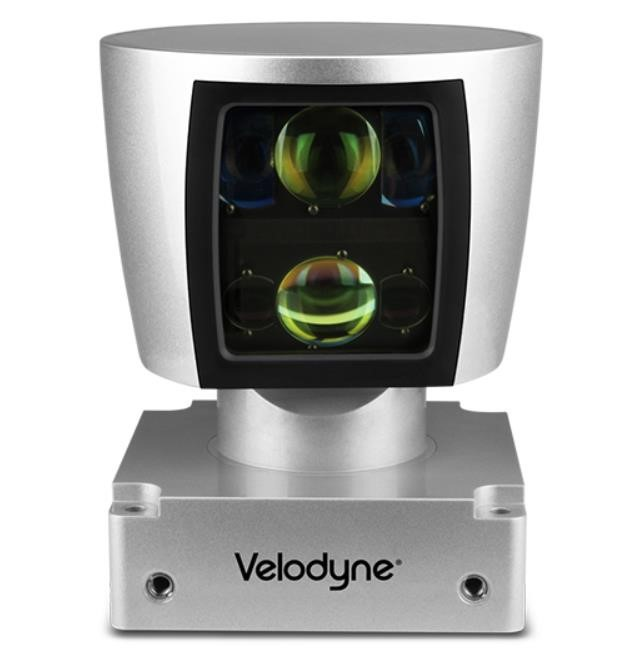
\includegraphics[width=\linewidth]{../figures/imgs/lidar.jpg}\end{minipage} & \begin{minipage}{0.15\textwidth}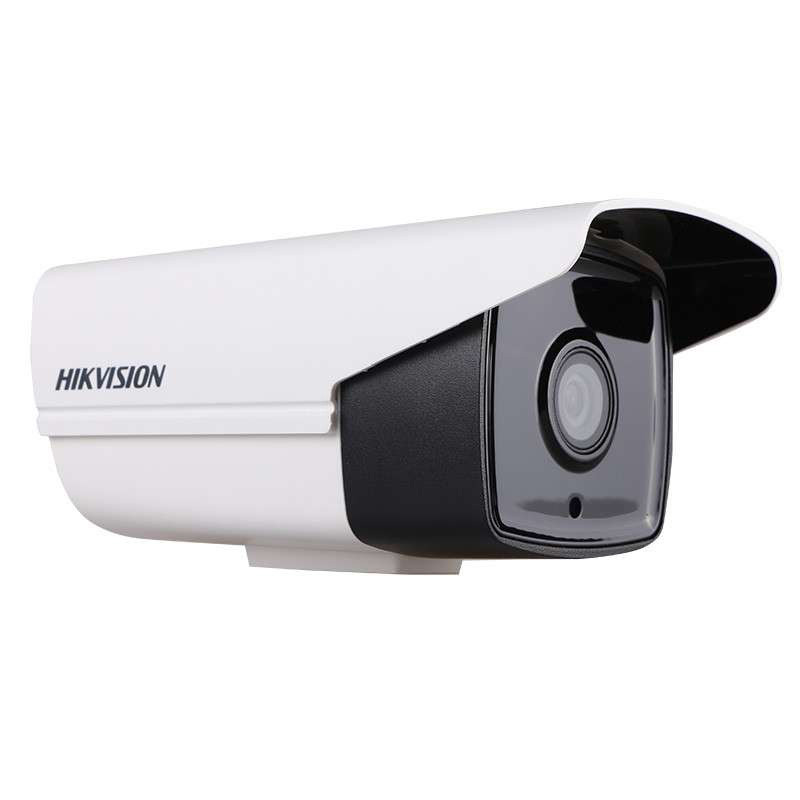
\includegraphics[width=\linewidth]{../figures/imgs/camera.jpg}\end{minipage} & \begin{minipage}{0.15\textwidth}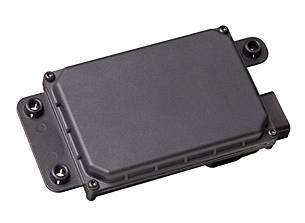
\includegraphics[width=\linewidth]{../figures/imgs/mlidar.jpeg}\end{minipage} \\ \hline
			价格      & 8000美元以上    & 35-50美元         & 300-500美元    \\ \hline
			优点      & \makecell*[c]{扫描周围环境得到精确\\环境信息、距离信息}   & \makecell*[c]{成本比较低,通过算法\\可以实现各种功能} & \makecell*[c]{不受天气影响,\\测量精度高}  \\ \hline
			缺点      & \makecell*[c]{成本高,大雾、雨雪天气\\效果差,无法图像识别}  & \makecell*[c]{恶劣环境下失效,难以测距,\\探测距离较近,算法要求高}   & \makecell*[c]{无法识别道路指示牌,\\无法识别行人}   \\ 
			\bottomrule[1.5pt]
	\end{tabular}}
	\label{table:sensor_cmp}
\end{table}
